\documentclass[11pt,a4paper]{article}
 
\usepackage{polski}
\usepackage[utf8]{inputenc} %utf-8 żeby nie było problemów z przenoszeniem między windowsem a linuxem
\usepackage{graphicx}
\usepackage{listings}
\usepackage{indentfirst}

%lokalne makro na komendę
\newcommand{\HRule}{\rule{\linewidth}{0.5mm}}

\setlength\parindent{24pt}
\oddsidemargin=20pt
\textwidth=420pt



 
\begin{document}

%strona tytułowa
\begin{titlepage}
\begin{center}
%nagłówek uczelni
\textsc{\LARGE Politechnika Warszawska}\\[0.5cm]
\textsc{\Large Wydział Elektroniki i Technik Informacyjnych}\\
\textsc{\Large Instytut Automatyki i Informatyki Stosowanej}\\[1.5cm]

\textsc{\Large Praca inżynierska} \\[0.5cm]
%tytuł między kreskami
\HRule \\[0.4cm]
{ \huge \bfseries Generator raportów z baz danych w technologii XSL-FO  bazujący na wzorcach \\[0.4cm]}
\HRule \\[1.5cm]

%autor
\begin{minipage} {0.4\textwidth}
\begin{flushleft} \large
\emph{Autor:}\\
 Maciej Kucharski 
\end{flushleft}
\end{minipage}
%promotor
\begin{minipage} {0.4\textwidth}
\begin{flushright} \large

\emph{Opiekun:}\\
doc. dr inż. Tomasz Traczyk

\end{flushright}
\end{minipage}	
\vfill
\large Semestr 13Z

	\end{center}
\end{titlepage}
 
\tableofcontents
\newpage

%Wstęp
\section{Wstęp} \label{sec:wst}
Obecnie bazy danych wykorzystywane są powszechnie. Niemal każde przedsiębiorstwo dysponujące przynajmniej podstawową infrastrukturą informatyczną wykorzystuje w swoich działaniach bazę danych. Dane zgromadzone w takiej bazie danych często muszą być przedstawiane, np. zarządowi przedsiębiorstwa, bądź udostępniane publiczne w przypadku instytucji publicznych. Zwykła, surowa tabela będąca wynikiem działania zapytania \emph{SQL} nie jest wystarczająca dla takich zastosowań ze względu na jej ubogi wygląd oraz kiepską czytelność.  Samo pobieranie raportowanych danych z bazy również jest problematyczne ze względu na konieczność znajomości języka \emph{SQL}. 

Funkcjonalny z punktu widzenia biznesu system raportowy powinien spełniać pewne wymagania:
\begin{itemize}
	\item umożliwienie stosowania własnych wzorców wyglądu raportu (tzw. \emph{layout})
	\item minimalizacja wymaganej ilości wiedzy informatycznej w celu określania danych przeznaczonych do raportu
	\item umożliwienie generowania raportów w formacie \emph{PDF} w celu uniknięcia problemów wynikających z wykorzystywania różnych platform systemowych
\end{itemize}

Na rynku dostępna jest cała gama narzędzi spełniających powyższe wymagania w mniejszym lub większym stopniu. Najlepszym przykładem jest \emph{Oracle BI Publisher}, który spełnia wszystkie wyżej postawione wymagania, jednak konieczność corocznego ponoszenia niemałych kosztów wynikających z opłat licencyjnych sprawia, że jest on w zasięgu niewielu organizacji.

Alternatywą jest darmowy \emph{Oracle Application Express}, zwany również \emph{ApEx'em}, instalujący się wraz z bazą danych \emph{Oracle}. Standardowo generowane przez \emph{ApEx} raporty nie są zby zaawansowane graficznie. Celem niniejszej pracy jest opracowanie rozwiązań zwiększających jego możliwości.

W ramach pracy przygotowano:
\begin{itemize}
	\item narzędzie generujące arkusz przekształceń \emph{XSLT} na podstawie danych wejściowych i wzorca wyglądu raportu
	\item przykładową konfigurację \emph{ApEx}
	\item przykładowe wzorce wyglądu raportu w celu demonstracji
\end{itemize}


\newpage

\section{Wprowadzenie teoretyczne} \label{sec:teoria}
Raport jest standardową formą dokumentu biznesowego, który służy do logicznej prezentacji informacji jakościowych oraz ilościowy. Raporty, w zależności od swojego zastosowania, mogą zawierać różne informacje, stąd też przedstawione na nich informacje mogą być przeznaczone dla różnych grup odbiorców. Również układ wizualny raportu powinien być dostosowany do odbiorcy - raport przygotowany dla celów operacyjnych nie musi mieć atrakcyjnej szaty graficznej, w przeciwieństwie do raportu przeznaczonego dla kierownictwa organizacji, bądź wglądu publicznego. 

Funkcjami raportów to np. podsumowywanie kluczowych wskaźników biznesu, prezentacja miar biznesowych w oparciu o rozmaite statystyki, czy ocena wydajności biznesowej, umożliwiająca szybką weryfikację stopnia realizacji strategicznych celów przedsiębiorstwa. Ze względu na swoje funkcje, raporty należą do najważniejszych dokumentów, którymi dysponuje organizacja. 
Za raport może być uznany każdy dokument prezentujący jakieś dane w ustandaryzowany sposób, jednak w ramach niniejszej pracy ograniczono się do podstawowych typów raportów najczęściej występujących w literaturze. Zostaną one zaprezentowane w dalszej części rozdziału.

\subsection{Raport typu \emph{master-detail}} \label{teoria:md}
Ten typ raportu służy prezentacji wartości pełniących funkcję nadrzędnych względem innych oraz szczegóły aktualnie wybranej pozycji. Najlepszym przykładem raportu tego typu jest powszechnie występujący dokument, jakim jest np. faktura. Ten typ raportu może być zastosowany przy występowaniu związków typu jedne-wiele. Zarówno obszar nadrzędny, jak i podrzędny może być listą lub drzewem pozycji, co umożliwia wprowadzenie wielu stopni podrzędności. Obszar podrzędny zwykle jest prezentowany pod obszarem nadrzędnym lub obok niego. Przykładem może być wspomniana uprzednio faktura prezentująca spis pozycji wchodzących w skład zamówienia lub spis pracowników zatrudnionych w konkretnym dziale spółki. Przykładowa faktura zaprezentowana jest na rysunku \ref{img:faktura}. Dane klienta i numer faktury są uznawane za dane nadrzędne, zaś pozycje występujące na fakturze - podrzędne. 

%źródło
%http://www.infakt.pl/images/icons-for_articles/grafiki/faktura_vat_pdf.png
\begin{figure}[h]
\centering
\caption{Faktura jako przykład raportu \emph{master-detail}}
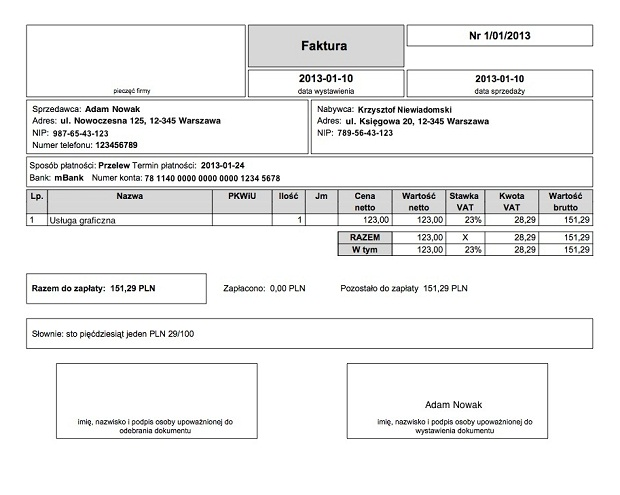
\includegraphics[scale=0.80]{faktura_vat_pdf}
\label{img:faktura}
\end{figure}

\subsection{Raport z grupami łamiącymi ( \emph{break-groups} )} \label{teoria:bg}
Głównym celem tego typu raportu jest zwiększenie jego czytelności. Polega na podziale wierszy trafiających do raportu na grupy o odpowiednich wartościach w wyróżnionych kolumnach. Każda z takich grup może zostać odpowiednio obsłużona, np. poprzez opatrzenie ich nagłówkami, wyliczenie dla nich podsumowań itp. Taka struktura umożliwia dość elastyczną prezentację tych samych danych. Grupy łamiące mogą być zastosowane w innych typach raportów, np. wspomnianym w rozdziale \ref{teoria:md} raporcie \emph{master-detail}. Na obrazku \ref{img:bg} zaprezentowany jest przykład raportu wykorzystującego grupy łamiące. Dane przedstawione na nim są zgrupowane według dwóch pierwszych kolumn.
%źródło
%http://docs.oracle.com/cd/E17904_01/bi.1111/b32122/img/grp1col_lft1_out1.gif
\begin{figure}[h]
\centering
\caption{Przykład raportu wykorzystującego grupy łamiące}
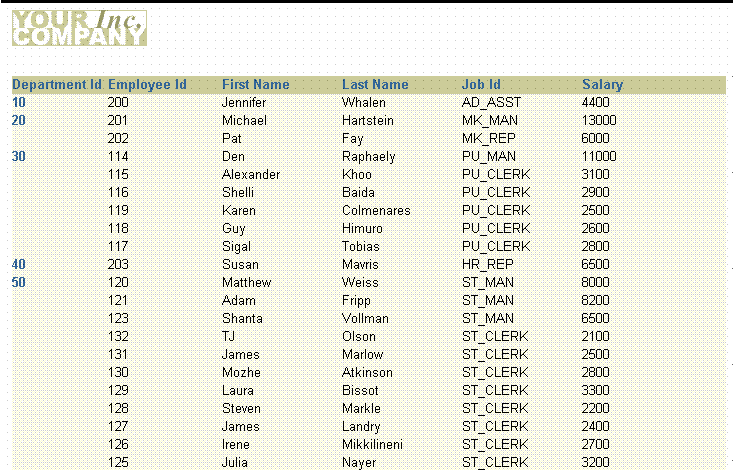
\includegraphics[scale=0.7]{grp1col_lft1_out1}
\label{img:bg}
\end{figure}

\subsection{Raport macierzowy ( krzyżowy) } \label{teoria:ct}
Raport macierzowy jest wykorzystywany do prezentacji związków między dwoma wymiarami. Raporty tego typu są często wykorzystane do analizy różnego rodzaju ankiet. Raport taki przedstawia związek między dwoma zmiennymi, tym samym ułatwiając znalezienie zależności między nimi. Struktura raportu tego typu może być porównana do wyglądu arkusza kalkulacyjnego z programu \emph{MS Excel}. W szczególności w ten sposób można raportować dane między którymi nie ma jawnej zależności. Przykład raportu macierzowego jest przedstawiony na rysunku \ref{img:ct}. Prezentuje on sprzedaż pewnych produktów w poszczególnych latach. 

%źrodło: http://doc.windev.com/en-US/images/image.awp?langid=3&name=etatTableaucroise3.gif&-1373238303
\begin{figure}[h]
\centering
\caption{Przykład raportu macierzowego}
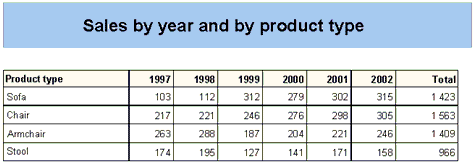
\includegraphics[scale=1]{crosstab_report}
\label{img:ct}
\end{figure}

\newpage

%Narzędzia
\section{Wykorzystane narzędzia i technologie} \label{sec:tools}
Pomimo pozornej prostoty raportowania, proces ten wykorzystuje wiele rozmaitych standardów oraz już istniejących narzędzi. Najważniejsze z nich zostaną pokrótce przedstawione w następujących podrozdziałach.

\subsection{Oracle Application Express (ApEx)} \label{tools:apex}
Oracle Application Express, zwany również ApEx'em, jest darmowym narzędziem instalującym się wraz z bazą danych firmy \emph{Oracle}. Umożliwia ono zarówno szybkie tworzenie strony raportowych, jak i bardziej skomplikowanych aplikacji bez programowania. Posiada wbudowany kreator zapytań \emph{SQL}, dzięki czemu osoba z minimalnym przygotowaniem informatycznym jest w stanie określić odpowiednie zapytanie pobierające dane z bazy. \emph{ApEx} nie posiada jednak wbudowanego mechanizmu pozwalającego na tworzenie wydruków w formacie \emph{PDF}. W tym celu należy skorzystać z zewnętrznego narzędzia. Jednym z nich może być Oracle BI Publisher, jednak nie jest to narzędzie tanie, a poza tym samo w sobie jest kompletnym systemem raportowym, a zatem w przypadku jego posiadania, stosowanie ApEx'a jest zbędne. Alternatywą jest wykorzystanie Apache FOP. Jest to darmowe narzędzie pozwalające na generowanie plików w formacie \emph{PDF}. Poglądowy schemat wykorzystania FOP przez ApEx'a jest zaprezentowany na obrazku 
\ref{img:apex_fop}. Pierwszym krokiem do wygenerowania raportu jest zainicjowane tego procesu przez użytkownika końcowego. Pośredniczy w tym osadzony na bazie danych serwer HTTP, który odpowiada za funkcjonowanie ApExa. Przekazuje on żądanie do bazy danych, a ta z kolei za pomocą odpowiedniego pakietu \emph{PL/SQL} wysyła do kontenera serwletów, na którym jest uruchomione FOP dane w formacie XML oraz wzorzec wyglądu raportu, a dokładniej transformację XSLT odpowiadającą za stworzenie dokumentu w formacie XSL-FO poprzez przekształcenie danych w XML. W efekcie, wynikowy plik w formacie PDF jest zwracany do ApEx'a, a następnie przekazywany użytkownikowi końcowemu. 

%rozmieści się samo gdzieś
\begin{figure}[h]
\centering
\caption{Wykorzystanie FOP przez Oracle Application Express}
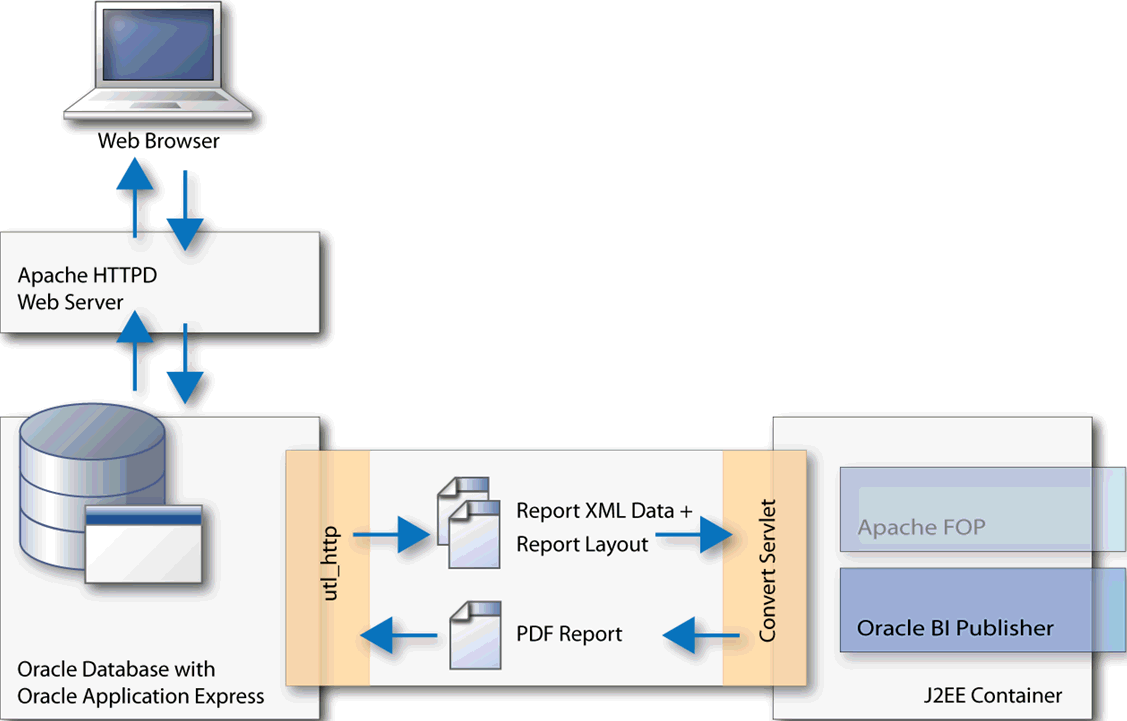
\includegraphics[scale=0.5]{apex_fop_usage}
\label{img:apex_fop}
\end{figure}

Ręczne tworzenie arkuszy XSLT dla potrzeb raportów jest jednak problematyczne. Zmiany we wzorcu wyglądu raportu pociągają za sobą konieczność dokonania zmian w transformacji XSLT. W przypadku drobnych zmian, takich jak np. zmiana marginesu bądź rozmiaru pewnego elementu problem nie jest jeszcze tak duży, jednak w przypadku konieczności np. dodania nowego elementu konieczne jest wykorzystanie specjalistycznej wiedzy. Ponadto stworzenie nowego wzorca od podstaw jest problematyczne dla osoby nie posiadającej wymaganych kompetencji.

Problem ten rozwiązuje jednak przygotowane w ramach pracy narzędzie. Potrafi ono, przy przyjęciu pewnych założeń, wygenerować arkusz transformacji XSLT na podstawie danych wejściowych oraz wzorca wyglądu raportu. Arkusz ten posłuży do przekształcenia danych w formacie XML w wynikowy raport w formacie XSL-FO. 

\subsection{XSLT} \label{tools:xslt}
XSLT (\emph{eXtensible Stylesheet Language Transformations} to oparty na XML język służący do przekstałcania jednych dokumentów w formacie XML na dowolny inny zgodny ze składnią XML. Jest podzbiorem szerszej specyfikacji określanej jako XSL. Transformacje XSLT zapisywane są w dokumentach XML z wykorzystaniem specjalnej przestrzeni nazw. Ze względu na dużą siłę wyrazu, łatwość implementacji oraz powszechne stosowanie XML, XSLT jest szeroko stosowane w różnych rodzajach oprogramowania. Ze względu na fakt, że współczesne przeglądarki internetowe posiadają wbudowane procesory XSLT, najczęstszym jego zastosowaniem jest transformacja dokumentów XML w celu wyświetlenia w przeglądarce WWW. Rysunek \ref{img:xslt} prezentuje poglądowy schemat zastosowania XSLT. W ramach niniejszej pracy XSLT jest stosowane do uzyskania raportu w formacie XSL-FO, co umożliwia stworzenie pliku PDF przez FOP.
\begin{figure}[h]
\centering
\caption{Schemat poglądowy zastosowania XSLT}
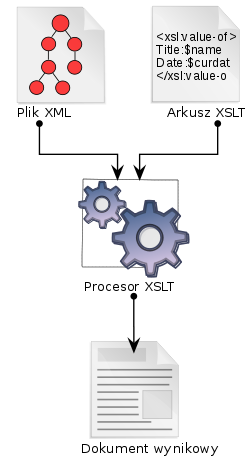
\includegraphics[scale=0.5]{xslt}
\label{img:xslt}
\end{figure}

\subsection{XSL-FO} \label{tools:xslfo}
XSL Formatting Objects to wykorzystujący XML język stosowany do formatowania dokumentów. Jest podzbiorem szerszej specyfikacji XSL. Dokumenty XSL-FO są zapisywane w XML z wykorzystaniem specjalnej przestrzeni nazw. Główną ideą powstania tej specyfikacji jest fakt, że w przeciwieństwie do HTML, czy XHTML, dokumenty XML nie posiadają wbudowanego układu wizualnego. XSL-FO jest językiem, który może zostać użyty do nadania dokumentowi XML układu na stronie, kolorów, czcionek itd. z przeznaczeniem wyniku dla różnych mediów, jak np. ekranu lub drukarki. W tym sensie pełni funkcję podobną do stylów CSS, jednak jest bardziej elastyczny i daje większe możliwości, zwłaszcza jeśli chodzi np. o stronicowanie i przewijanie. Główną różnicą między XSL-FO, a CSS jest fakt, że informacje o układzie wizualnym są zawarte w tym samym dokumencie, co dane. Rozdział danych od stylu można uzyskać np. przez zastosowanie transformacji XSLT do danych w XML.

\subsection{Apache FOP} \label{tools:fop}
Apache FOP (\emph{Formatting Objects Processor}) jest najpopularniejszym procesorem obiektów formatujących. Jest to darmowy program napisany w języku \emph{Java}, który konwertuje pliki zapisane w formacie XSL-FO na pliki w formacie PDF lub innych drukowalnych, m.in. RTF czy PostScript. FOP umożliwia również przetwarzanie danych w formacie XML przy użyciu odpowiednich transformacji XSLT. Najnowsza stabilna wersja nie jest w pełni zgodna ze specyfikacją XSL-FO 1.1, lecz najważniejsze elementy są wspierane.

FOP może być wykorzystywany zarówno jako niezależna aplikacja uruchamiana np. z wiersza poleceń, jak i biblioteka Javy, co umożliwia wykorzystanie w dowolnej aplikacji przeznaczonej do uruchamiania w środowisku maszyny wirtualnej Javy (\emph{JVM}). Dodatkowo, wraz z instalacją ApEx'a, dostarczane jest archiwum \emph{war} zawierające specjalnie przygotowaną wersję FOP przeznaczoną do uruchamiania na kontenerze serwletów. Domyślna konfiguracja nie wspiera jednak stosowania narodowych czcionek, np. polskich znaków, jednak jest to możliwe po pewnych zmianach konfiguracyjnych. 

W ramach pracy FOP jest wykorzystywane do generowania plików w formacie PDF.

\subsection{SVG} \label{tools:svg}
SVG (\emph{Scallable Vector Graphics}) to bazujący na XML format do zapisu dwuwymiarowej grafiki wektorowej. Jest to otwarty standard utworzony przez organizację W3C. Standard jest powszechnie wspierany przez współczesne przeglądarki internetowe, z myślą o których powstał. Może jednak być również wykorzystywany jako niezależny od platformy systemowej format grafiki wektorowej. Za pomocą SVG można tworzyć zarówno statyczne grafiki, jak i animacje.

Plik zawierający grafikę SVG może być edytowany dowolnym edytorem tekstowym, jednak wygodniejsze jest zastosowanie do tego celu dedykowanego oprogramowania. Polecanym do tego celu programem jest darmowy \emph{InkScape}.

W ramach pracy standard SVG jest wykorzystywany do zapisu wzorca wyglądu raportu. 
\newpage


%Koncepcja
\section{Proponowane rozwiązanie problemu} \label{sec:solution}
\subsection{Ogólna koncepcja} \label{solution:koncept}
Głównym problemem przy wykorzystaniu ApEx'a jest konieczność tworzenia nowych arkuszy transformacji XSLT przy zmianach wzorca wyglądu raportu. Przy wykorzystaniu przez biznes jest to niedopuszczalne. W związku z tym w ramach pracy zostało przygotowane narzędzie mające na celu rozwiązanie tego problemu. Jego głównym przeznaczeniem jest wspieranie ApEx'a w zakresie generowania arkuszy transformacji XSLT na podstawie danych wejściowych w XML oraz wzorca wyglądu raportu w SVG. Arkusz ten może być wykorzystany do przekształcenia pliku XML z danymi w plik w formacie XSL-FO. Ten z kolei może zostać wysłany do FOP, co skutkuje utworzeniem raportu w formacie PDF.

\subsection{Dane wejściowe} \label{solution:data}
Dane przeznaczone do raportu zapisane są w formacie XML. Ponieważ dane pochodzą z ApEx'a, możliwe jest przyjęcie założeń odnośnie ich struktury. Ogólna struktura jest przedstawiona na listingu \ref{rap:apex}. Element ROWSET jest opcjonalny i może nie wystąpić. Wpis zawierający informacje zawarte w pojedynczym wierszu zawarte są w strukturze znacznika ROW. W nim z kolei znajdują się informacje dotyczące poszczególnych kolumn. Nazwa kolumny jest taka sama, jak nazwa znacznika, zaś wartość odpowiadająca węzłowi to wartość konkretnej danej.

\lstset{language=XML}
\begin{lstlisting}[frame=single,caption=Ogólna postać dokumentu XML z danymi pochodzącymi z ApExa,label=rap:apex]
<?xml version="1.0" encoding="UTF-8"?>
<DOCUMENT>
 <REGION ID="">
  <ROWSET>
   <ROW>
    <KOLUMNA1>...</KOLUMNA1>
    <KOLUMNA2>...</KOLUMNA2>
       ...	
   </ROW>
   <ROW>....</ROW>
  </ROWSET>
 </REGION>
</DOCUMENT>
\end{lstlisting}

Ponadto, w pliku danych mogą zostać przekazane dodatkowe informacje. Mogą to być np. informacje o zalogowanym użytkowniku, sesji, identyfikator aplikacji, data itp. Można również przekazać inne informacje znajdujące się w pewnym miejscu na stronie w ApEx'ie. Jest to tzw. \emph{region}. Fakt ten jest wykorzystywany do przekazania informacji ,,nadrzędnych" przy wyborze raportu typu \emph{master-detail}. Format danych ,,nadrzędnych" jest zaprezentowany na listingu \ref{rap:master}. Dane te zawarte są w strukturze głównego znacznika DOCUMENT. Litera X w widocznym przykładzie jest w rzeczywistości numerem strony w ApEx'ie, na której znajduje się owa dana. Litera P występuje zawsze. 

\lstset{language=XML}
\begin{lstlisting}[frame=single,caption=Format danych typu \emph{master},label=rap:master]
<?xml version="1.0" encoding="UTF-8"?>
<DOCUMENT>
 <PX_DANA1>...</PX_DANA1>
 <PX_DANA2>...</PX_DANA2>
 ...
</DOCUMENT>
\end{lstlisting}

Dodatkowym założeniem mającym na celu uproszczenie stosowania grup łamiących w raportach jest wymaganie, by zapytanie \emph{SQL} pobierające dane do raportu posiadało klauzulę \emph{ORDER BY} sortującą dane według wyróżnionych kolumn. Rzeczywisty przykład danych wejściowych jest przedstawiony na listingu \ref{rap:complete}.

\lstset{language=XML}
\begin{lstlisting}[frame=single,caption=Przykładowe dane,label=rap:complete]
<?xml version="1.0" encoding="UTF-8"?>
<DOCUMENT>
 <P8_DEPTNAME>Accounting</P8_DEPTNAME>
 <P8_DESCR>Department description</P8_DESCR>
   <ROWSET>
    <ROW>
      <JOB>PRESIDENT</JOB>
      <ENAME>KING</ENAME>
      <HIREDATE>11/17/1981</HIREDATE>
      <SAL>5000</SAL>
      <COMM/>
      <MGR/>
    </ROW>
   </ROWSET>
</DOCUMENT>
\end{lstlisting}

\subsection{Wzorzec wyglądu raportu} \label{solution:layout}
Wzorzec wyglądu raportu jest zapisany w formacie SVG, jak zostało to zaznaczone w rozdziale \ref{tools:svg}. Specyfikacja SVG zawiera bardzo dużo elementów. W ramach pracy nie byłoby możliwe pełne wsparcie specyfikacji, zatem przyjęto pewne ograniczenia. Wspieranymi elementami jest stały tekst, grafika (np. logo organizacji) oraz prostokąty jako pola danych.

Kolejne założenie upraszczające dotyczy reprezentacji tabeli. W SVG nie występuje specjalna konstrukcja służąca do tworzenia tabeli. Jest ona reprezentowana za pomocą odpowiednio rozmieszczonych prostokątów. Przyjmuje się, że wzorzec jest stworzony za pomocą programu \emph{InkScape} z dołączonym pluginem odpowiedzialnym za tworzenie tabel. Dodaje on do kwadratów tworzących tabelę dodatkowe atrybuty \emph{inkex:row} oraz \emph{inkex:column} co w znacznym stopniu ułatwia przetwarzanie wzorca.

\end{document}

